\documentclass[11pt]{article}

\RequirePackage[l2tabu, orthodox]{nag}
%\documentclass{article}

\usepackage[left=1.25in, right=1.25in, top=1.25in, bottom=1.25in]{geometry}

% FONTS
%\usepackage[T1]{fontenc}

% Replace default Latin Modern typewriter with its proportional counterpart
% http://www.tug.dk/FontCatalogue/lmoderntypewriterprop/
%\renewcommand*\ttdefault{lmvtt}


%%% OPTION 1 - Fourier Math + New Century Schoolbook + ParaType Sans

% % Import Fourier Math (this imposes its own New Century Schoolbook type)
% % http://www.ctan.org/tex-archive/fonts/fouriernc/
%\usepackage{fouriernc}
%\usepackage{amsmath}
% % Replace with TeX Gyre Schola version of New Century Schoolbook (must scale!)
% % http://www.tug.dk/FontCatalogue/tgschola/
%\usepackage[scale=0.92]{tgschola}
%\usepackage[scaled=0.88]{PTSans}

%% OPTION 2 - MathDesign Math + Bitstream Charter + ParaType Sans

% Import MathDesign (this brings along Bitstream Charter)
% http://www.ctan.org/tex-archive/fonts/mathdesign/
\usepackage[bitstream-charter]{mathdesign}
 \usepackage{amsmath}
\usepackage[scaled=0.92]{PTSans}


% %%% OPTION 3 - MTPRO 2 Math + Termes Times + ParaType Sans

% \usepackage{tgtermes}
% \usepackage{amsmath}
% \usepackage[subscriptcorrection,
%             amssymbols,
%             mtpbb,
%             mtpcal,
%             nofontinfo  % suppresses all warnings
%            ]{mtpro2}
% \usepackage{scalefnt,letltxmacro}
% \LetLtxMacro{\oldtextsc}{\textsc}
% \renewcommand{\textsc}[1]{\oldtextsc{\scalefont{1.10}#1}}
% \usepackage[scaled=0.92]{PTSans}

% Use default fonts here
\usepackage{amsmath}
%\usepackage{amssymb}

% COLOR
\usepackage[usenames,dvipsnames]{xcolor}
\definecolor{shadecolor}{gray}{0.9}

% SPACING and TEXT
\usepackage[final,expansion=alltext]{microtype}
\usepackage[english]{babel}
\usepackage[parfill]{parskip}
\usepackage{afterpage}
\usepackage{framed}
\usepackage{verbatim}
\usepackage{setspace}

%redefine the leftbar environment to accept a width and coloring options
\renewenvironment{leftbar}[1][\hsize]
{%
  \def\FrameCommand
  {%
    {\color{Gray}\vrule width 3pt}%
    \hspace{10pt}%
    %\hspace{0pt}\fboxsep=\FrameSep\colorbox{black!10}%
  }%
  \MakeFramed{\hsize#1\advance\hsize-\width\FrameRestore}%
}%
{\endMakeFramed}

% define a paragraph header function
\DeclareRobustCommand{\parhead}[1]{\textbf{#1}~}

% EDITING
% line numbering in left margin
\usepackage{lineno}
\renewcommand\linenumberfont{\normalfont
                             \footnotesize
                             \sffamily
                             \color{SkyBlue}}
% ragged paragraphs in right margin
\usepackage{ragged2e}
\DeclareRobustCommand{\sidenote}[1]{\marginpar{
                                    \RaggedRight
                                    \textcolor{Plum}{\textsf{#1}}}}
% paragraph counter in right margin
\newcommand{\parnum}{\bfseries\P\arabic{parcount}}
\newcounter{parcount}
\newcommand\p{%
    \stepcounter{parcount}%
    \leavevmode\marginpar[\hfill\parnum]{\parnum}%
}
% paragraph helper
%\DeclareRobustCommand{\PP}{\textcolor{Plum}{\P} }

% COUNTERS
\usepackage[inline]{enumitem}
\renewcommand{\labelenumi}{\color{black!67}{\arabic{enumi}.}}
\renewcommand{\labelenumii}{{\color{black!67}(\alph{enumii})}}
\renewcommand{\labelitemi}{{\color{black!67}\textbullet}}

% FIGURES
\usepackage{graphicx}
\usepackage[labelfont={it, small}, font=small]{caption}
\usepackage[format=hang]{subcaption}

% APPENDIX FIGURES
\usepackage{chngcntr}

% TABLES
\usepackage{booktabs}

% ALGORITHMS
\usepackage[algoruled]{algorithm2e}
\usepackage{listings}
\usepackage{fancyvrb}
\fvset{fontsize=\normalsize}

% THEOREMS
\usepackage{amsthm}
\newtheorem{proposition}{Proposition}
\newtheorem{lemma}{Lemma}

% BIBLIOGRAPHY
\usepackage{natbib}

% HYPERREF
\usepackage[colorlinks,linktoc=all]{hyperref}
\usepackage[all]{hypcap}
\hypersetup{citecolor=MidnightBlue}
\hypersetup{linkcolor=MidnightBlue}
\hypersetup{urlcolor=MidnightBlue}

% CLEVEREF must come after HYPERREF
\usepackage[nameinlink]{cleveref}

% ACRONYMS
\usepackage[acronym,smallcaps,nowarn]{glossaries}
% \makeglossaries

% COLOR DEFINITIONS
\newcommand{\red}[1]{\textcolor{BrickRed}{#1}}
\newcommand{\orange}[1]{\textcolor{BurntOrange}{#1}}
\newcommand{\green}[1]{\textcolor{OliveGreen}{#1}}
\newcommand{\blue}[1]{\textcolor{MidnightBlue}{#1}}
\newcommand{\gray}[1]{\textcolor{black!60}{#1}}

% LISTINGS DEFINTIONS
\lstdefinestyle{mystyle}{
    commentstyle=\color{OliveGreen},
    keywordstyle=\color{BurntOrange},
    numberstyle=\tiny\color{black!60},
    stringstyle=\color{MidnightBlue},
    basicstyle=\ttfamily,
    breakatwhitespace=false,
    breaklines=true,
    captionpos=b,
    keepspaces=true,
    numbers=left,
    numbersep=5pt,
    showspaces=false,
    showstringspaces=false,
    showtabs=false,
    tabsize=2
}
\lstset{style=mystyle}

\usepackage[colorinlistoftodos,
            prependcaption,
            textsize=small,
            backgroundcolor=yellow,
            linecolor=lightgray,
            bordercolor=lightgray]{todonotes}

% !TEX root = template.tex

% \DeclareRobustCommand{\mb}[1]{\ensuremath{\boldsymbol{\mathbf{#1}}}}
\DeclareRobustCommand{\mb}[1]{\boldsymbol{#1}}

% \newcommand{\KL}[2]{\ensuremath{\textrm{KL}\PARENS{#1\;\|\;#2}}}
\DeclareRobustCommand{\KL}[2]{\ensuremath{\textrm{KL}\left(#1\;\|\;#2\right)}}

\DeclareMathOperator*{\argmax}{arg\,max}
\DeclareMathOperator*{\argmin}{arg\,min}

\renewcommand{\mid}{~\vert~}
\newcommand{\given}{\,|\,}
\newcommand{\iid}[1]{\stackrel{\text{iid}}{#1}}

\newcommand{\mba}{\mb{a}}
\newcommand{\mbb}{\mb{b}}
\newcommand{\mbc}{\mb{c}}
\newcommand{\mbd}{\mb{d}}
\newcommand{\mbe}{\mb{e}}
\newcommand{\mbg}{\mb{g}}
\newcommand{\mbh}{\mb{h}}
\newcommand{\mbi}{\mb{i}}
\newcommand{\mbj}{\mb{j}}
\newcommand{\mbk}{\mb{k}}
\newcommand{\mbl}{\mb{l}}
\newcommand{\mbm}{\mb{m}}
\newcommand{\mbn}{\mb{n}}
\newcommand{\mbo}{\mb{o}}
\newcommand{\mbp}{\mb{p}}
\newcommand{\mbq}{\mb{q}}
\newcommand{\mbr}{\mb{r}}
\newcommand{\mbs}{\mb{s}}
\newcommand{\mbt}{\mb{t}}
\newcommand{\mbu}{\mb{u}}
\newcommand{\mbv}{\mb{v}}
\newcommand{\mbw}{\mb{w}}
\newcommand{\mbx}{\mb{x}}
\newcommand{\mby}{\mb{y}}
\newcommand{\mbz}{\mb{z}}

\newcommand{\mbA}{\mb{A}}
\newcommand{\mbB}{\mb{B}}
\newcommand{\mbC}{\mb{C}}
\newcommand{\mbD}{\mb{D}}
\newcommand{\mbE}{\mb{E}}
\newcommand{\mbF}{\mb{F}}
\newcommand{\mbG}{\mb{G}}
\newcommand{\mbH}{\mb{H}}
\newcommand{\mbI}{\mb{I}}
\newcommand{\mbJ}{\mb{J}}
\newcommand{\mbK}{\mb{K}}
\newcommand{\mbL}{\mb{L}}
\newcommand{\mbM}{\mb{M}}
\newcommand{\mbN}{\mb{N}}
\newcommand{\mbO}{\mb{O}}
\newcommand{\mbP}{\mb{P}}
\newcommand{\mbQ}{\mb{Q}}
\newcommand{\mbR}{\mb{R}}
\newcommand{\mbS}{\mb{S}}
\newcommand{\mbT}{\mb{T}}
\newcommand{\mbU}{\mb{U}}
\newcommand{\mbV}{\mb{V}}
\newcommand{\mbW}{\mb{W}}
\newcommand{\mbX}{\mb{X}}
\newcommand{\mbY}{\mb{Y}}
\newcommand{\mbZ}{\mb{Z}}

\newcommand{\mbalpha}{\mb{\alpha}}
\newcommand{\mbbeta}{\mb{\beta}}
\newcommand{\mbdelta}{\mb{\delta}}
\newcommand{\mbepsilon}{\mb{\epsilon}}
\newcommand{\mbchi}{\mb{\chi}}
\newcommand{\mbeta}{\mb{\eta}}
\newcommand{\mbgamma}{\mb{\gamma}}
\newcommand{\mbiota}{\mb{\iota}}
\newcommand{\mbkappa}{\mb{\kappa}}
\newcommand{\mblambda}{\mb{\lambda}}
\newcommand{\mbmu}{\mb{\mu}}
\newcommand{\mbnu}{\mb{\nu}}
\newcommand{\mbomega}{\mb{\omega}}
\newcommand{\mbphi}{\mb{\phi}}
\newcommand{\mbpi}{\mb{\pi}}
\newcommand{\mbpsi}{\mb{\psi}}
\newcommand{\mbrho}{\mb{\rho}}
\newcommand{\mbsigma}{\mb{\sigma}}
\newcommand{\mbtau}{\mb{\tau}}
\newcommand{\mbtheta}{\mb{\theta}}
\newcommand{\mbupsilon}{\mb{\upsilon}}
\newcommand{\mbvarepsilon}{\mb{\varepsilon}}
\newcommand{\mbvarphi}{\mb{\varphi}}
\newcommand{\mbvartheta}{\mb{\vartheta}}
\newcommand{\mbvarrho}{\mb{\varrho}}
\newcommand{\mbxi}{\mb{\xi}}
\newcommand{\mbzeta}{\mb{\zeta}}

\newcommand{\mbDelta}{\mb{\Delta}}
\newcommand{\mbGamma}{\mb{\Gamma}}
\newcommand{\mbLambda}{\mb{\Lambda}}
\newcommand{\mbOmega}{\mb{\Omega}}
\newcommand{\mbPhi}{\mb{\Phi}}
\newcommand{\mbPi}{\mb{\Pi}}
\newcommand{\mbPsi}{\mb{\Psi}}
\newcommand{\mbSigma}{\mb{\Sigma}}
\newcommand{\mbTheta}{\mb{\Theta}}
\newcommand{\mbUpsilon}{\mb{\Upsilon}}
\newcommand{\mbXi}{\mb{\Xi}}

\newcommand{\dif}{\mathop{}\!\mathrm{d}}
\newcommand{\diag}{\textrm{diag}}
\newcommand{\supp}{\textrm{supp}}

\newcommand{\E}{\mathbb{E}}
\newcommand{\Var}{\mathbb{V}\textrm{ar}}
\newcommand{\bbH}{\mathbb{H}}
\newcommand{\bbI}{\mathbb{I}}
\newcommand{\bbN}{\mathbb{N}}
\newcommand{\bbZ}{\mathbb{Z}}
\newcommand{\bbR}{\mathbb{R}}
\newcommand{\bbS}{\mathbb{S}}

\newcommand{\cA}{\mathcal{A}}
\newcommand{\cB}{\mathcal{B}}
\newcommand{\cC}{\mathcal{C}}
\newcommand{\cD}{\mathcal{D}}
\newcommand{\cE}{\mathcal{E}}
\newcommand{\cF}{\mathcal{F}}
\newcommand{\cG}{\mathcal{G}}
\newcommand{\cH}{\mathcal{H}}
\newcommand{\cI}{\mathcal{I}}
\newcommand{\cJ}{\mathcal{J}}
\newcommand{\cK}{\mathcal{K}}
\newcommand{\cL}{\mathcal{L}}
\newcommand{\cM}{\mathcal{M}}
\newcommand{\cN}{\mathcal{N}}
\newcommand{\cO}{\mathcal{O}}
\newcommand{\cP}{\mathcal{P}}
\newcommand{\cQ}{\mathcal{Q}}
\newcommand{\cR}{\mathcal{R}}
\newcommand{\cS}{\mathcal{S}}
\newcommand{\cT}{\mathcal{T}}
\newcommand{\cU}{\mathcal{U}}
\newcommand{\cV}{\mathcal{V}}
\newcommand{\cW}{\mathcal{W}}
\newcommand{\cX}{\mathcal{X}}
\newcommand{\cY}{\mathcal{Y}}
\newcommand{\cZ}{\mathcal{Z}}

\newcommand{\trans}{\mathsf{T}}
\newcommand{\naturals}{\mathbb{N}}
\newcommand{\reals}{\mathbb{R}}

\newcommand{\distNormal}{\mathcal{N}}
\newcommand{\distGamma}{\mathrm{Gamma}}
\newcommand{\distBernoulli}{\mathrm{Bern}}
\newcommand{\distBinomial}{\mathrm{Bin}}
\newcommand{\distCategorical}{\mathrm{Cat}}
\newcommand{\distDirichlet}{\mathrm{Dir}}
\newcommand{\distMultinomial}{\mathrm{Mult}}
\newcommand{\distPolyaGamma}{\mathrm{PG}}
\newcommand{\distMNIW}{\mathrm{MNIW}}
\newcommand{\distPoissonProcess}{\mathrm{PP}}

\newcommand{\dtmax}{\Delta t_{\mathsf{max}}}

\newacronym{KL}{kl}{Kullback-Leibler}
\newacronym{ELBO}{elbo}{\emph{evidence lower bound}}
\newacronym{POPELBO}{pop-elbo}{\emph{population evidence lower bound}}

\newacronym{SVI}{svi}{stochastic variational inference}
\newacronym{BUMPVI}{bump-vi}{bumping variational inference}

\newacronym{GMM}{gmm}{Gaussian mixture model}
\newacronym{LDA}{lda}{latent Dirichlet allocation}

\newacronym{SUTVA}{sutva}{stable unit treatment value assumption}


\newcommand{\celegans}{\textit{C. elegans}}

% \title{\large Discrete and continuous latent states of neural activity in \textit{Caenorhabditis elegans}}
% \title{Hierarchical recurrent models reveal latent states of neural activity in \textit{C. elegans}}
\title{Hierarchical state space models reveal dynamics of neural activity in \textit{C. elegans}}
\author{Scott Linderman$^{\text{1}}$,
  Annika Nichols$^{\text{2}}$,
  David Blei$^{\text{1}}$,
  Manuel Zimmer$^{\text{2}}$,
  and
  Liam Paninski$^{\text{1}}$
  \\
  $^{\text{1}}$Columbia University,
  $^{\text{2}}$Research Institute of Molecular Pathology (IMP), Vienna Biocenter
}

\begin{document}

\doublespacing

\maketitle

\begin{abstract}
  Recent advances in neural recording technologies enable
  simultaneous measurements of the majority of head ganglia neurons in
  both immobilized and freely-behaving
  \celegans~\citep{schrodel2013brain, prevedel2014simultaneous,
    nguyen2016whole}.  The dynamics of neural activity shed light on
  how \celegans~processes sensory information and generates motor
  activity.  To understand these dynamics, we develop recurrent state
  space models that decompose complex time-series into segments with
  simple, linear dynamics. We incorporate these models into a
  hierarchical framework for combining information across whole-brain
  recordings of many worms.  Using this framework, we reveal latent
  states of population neural activity, along with the discrete
  behavioral ``syllables'' that drive dynamics in this latent state
  space.  We find stochastic transition patterns between these
  syllables, and we see that transition probabilities are determined
  by both current brain state and environmental cues.  In
  addition to quantifying neural dynamics, this probabilistic
  framework aids in neural identification---currently a laborious,
  manual task---and reveals clusters of neurons that are similarly
  tuned in latent state space.  Finally, we find a significant overlap
  between our inferred syllables and the manually-labeled states
  of~\citet{kato2015global} and~\citet{nichols2017global}, which were
  shown to correspond to different behaviors, like forward crawling,
  reversals, and turns. Our methods automatically discover and
  quantify these states directly from neural
  activity, yielding powerful new tools for neuro-behavioral analysis.
\end{abstract}

\clearpage

\section*{Introduction}

\textbf{Context:}
\begin{itemize}
\item Novel recording technologies enable simultaneous recording of
  O(100) of neurons simultaneously.  In \celegans, this constitutes
  the bulk of the head ganglia, and in other organisms this may constitue
  the majority of neurons in a specific circuit.
\item The promise is that these new recordings will lead to new
  insights into brain function. For example, with a complete view of a
  circuit, we should be able to study how it responds to external
  inputs, how it represents its internal state, and how it transforms
  internal states into circuit outputs.
\item \celegans~is the ideal model organism for realizing
  this goal.  It has a stereotyped nervous system with 302 identifiable
  neurons.  Its head ganglia is responsible for
  processing sensory inputs and generating outputs that initiate
  motor commands, like forward crawling, reversals, and turns.
\item With new recording capabilities, we can study how the
  coordinated activity of the \celegans~head ganglia encodes internal
  state, updates it in response to sensory information (like oxygen
  concentration), and transmits it via output (motor) neurons.
\item Moreover, we can study how the encoding, dynamics, and outputs
  differ across individual worms, genetic strains, and developmental stages.
\end{itemize}


\textbf{Three Problems: How to conceptualize the latent states of
  brain activity, their dynamics, and their relation to observed
  activity?  How to learn these dynamics from partial recordings of
  many individual worms? How to quantify differences between worms of
  different genetic strains and developmental stages?}
\begin{itemize}
\item We seek a model that is flexible enough to capture the complexity
  of neural dynamics and the relationship between latent states and
  observed activity, but we also require that the model be composed
  of interpretable building blocks. 
\item We have a spectrum of options --- simple factor analyzers and
  clustering algorithms, to Kalman filters and hidden Markov models,
  all the way up to highly nonlinear neural network models.
\item The challenge is to strike a balance: flexible yet interpretable.
\item While, in aggregate, we have a great deal of data to fit these models
  with, the recordings are spread over many individuals. In
  each individual we can only label a handful of neurons and we only
  record them for tens of minutes (photobleaching).
\item Moreover, each individual has its own idiosyncrasies due to
  factors like different levels of GCaMP expression from one worm
  to another, as well as subtle differences in the underlying brain
  dynamics. 
\item We need methods that combine these limited, partial recordings
  in order to learn shared structure shared across the population.
\item Finally, in order to understand the differences between
  genetic strains and developmental stages, we need models that allow
  us to flexibly test hypotheses about how they differ. 
\end{itemize}


\textbf{Main results, in broad brushstrokes:}
\begin{itemize}
\item We build a probabilistic framework for learning sophisticated neural dynamics from populations of worms.
  % The framework is:
  % \begin{itemize}
  % \item \emph{hierarchical}, capturing canonical structure while allowing variability across worms, genetic strains, and developmental stages;
  % \item \emph{robust}, ameliorating some concerns of model misspecification;
  % \item \emph{recurrent}, capturing nuances in the co-evolution of discrete and continuous latent states;
  % \item \emph{input-driven}, capturing the influence of exogenous factors and sensory inputs;
  % \item and most importantly, \emph{composed} of simple and interpretable pieces that shed light on the dynamics of neural activity.
  % \end{itemize}
\item We use this framework to extract low-dimensional state
  trajectories for each worm, using shared correlations across the
  population to align the trajectories and make predictions about
  unseen activity.
\item We discover clusters of similarity-tuned and highly correlated
  neurons, and we find that these neurons are functionally grouped
  according the different behaviors they are implicated in.
\item We show how our model's predictions can aid in identifying neurons (which will then drive down posterior uncertainty in the underlying dynamics of neural activity).
\item We show that brain dynamics are well-approximated as switching between discrete regimes, or ``syllables,'' each associated with simple linear dynamics.  These syllables map onto the manual segmentations of experimental experts, which were based on known behavioral implications of certain patterns of brain activity.
\item We quantify these linear dynamical regimes, show how they drive activity in clusters of neurons, and evaluate their differences from worm to worm.
\item We find that transitions between syllables are not simply Markovian; rather, the transitions depend on a combination of syllable history and latent brain state.
\item We measure how oxygen concentration (and change in oxygen concentration) differentially impact state transitions in worms of different genetic strains and developmental stages, and we find that sudden increases in oxygen elicit a characteristic, transient response regardless of genetic make-up or developmental stage, but that only certain genetic strains show a sustained response to increased oxygen levels. 
\end{itemize}


\clearpage

\section*{Results}

\subsection*{A probabilistic framework that combines information across
  trials to learn canonical dynamics}


\begin{figure}[t!]
\centering%
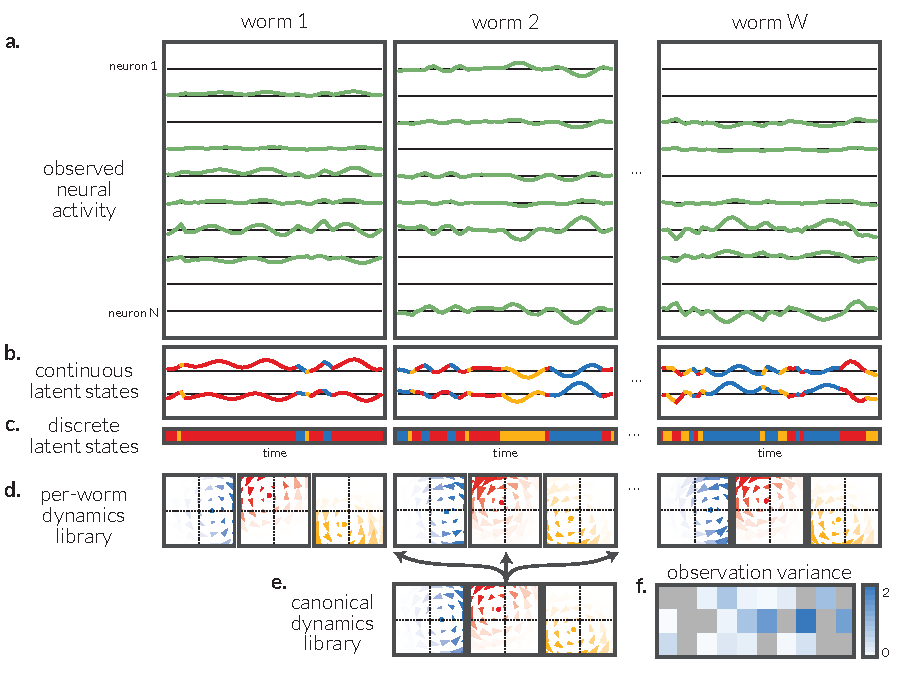
\includegraphics[width=6in]{figures/v4/figure1} 
\caption{
  \textit{A probabilistic framework for combining
  information across multiple worms in order to learn a shared
  dynamics model for \celegans.}
  \textbf{a.}~The data consists of observed neural activity collected
  from many different worms.  In each recording we observe a different
  subset of labeled neurons in the head ganglia.
  \textbf{b.}~We model the observed activity as a linear function of
  an underlying, continuous, and typically low-dimensional latent state,
  here shown as a two-dimensional signal for each recording.
  \textbf{c.}~The dynamics of these continuous states are governed by
  a co-evolving discrete state, or \emph{syllable}.
  \textbf{d.}~These syllables index into a library of linear
  dynamics functions for each worm, here shown as maps from~$\reals^2$ to~$\reals^2$.
  Each dynamics function is selectively used in different regions of
  continuous latent space, as shown by the different intensities of
  the vector field.
  \textbf{e.}~Though location in continuous state space helps inform
  transitions, the current syllable does as well. This is captured
  by a Markov transition matrix, which is modulated by location in
  continuous state space.
  \textbf{f.}~To increase robustness to model misspecification, we
  use a multivariate-t distribution for the noise in the continuous
  state updates.
  \textbf{g.}~Each worm has its own dynamics library, but they are
  constrained to be close to the shared, canonical library.  This
  combines information to learn shared structure while also allowing
  for worm-to-worm variability.
  \textbf{h.} Likewise, we allow each worm to have its own observation
  variances to account for individual differences that may arise from,
  for example, variable levels of fluorescent protein expression.
  Missing neurons are denoted by gray boxes. 
}
\label{fig:model}
\end{figure}

We seek a parsimonious characterization of the dynamics of neural
activity in the head ganglia of \celegans. Recent advances in optical
imaging offer simultaneous recordings of most of the head ganglia
neurons, but we must surmount three main challenges in order to learn
a dynamics model from these data.  First, we need to design a model
flexible enough to capture nonlinear dynamics yet interpretable enough
to reveal simplifying structure when it exists.  Moreover, any model
will necessarily be an approximation to the true neural dynamics, and
as such we need to be robust to data that does not quite match model
predictions.  Finally, our model must combine partial recordings from
separate organisms to learn shared neural dynamics yet still allow for
individual variability. We construct a recurrent, robust, and
hierarchical state space model that addresses these challenges,
decomposing complex dynamics into a collection of simpler pieces that
can be learned from noisy, partial recordings with trial-to-trial
variability.  We call this model \textbf{TBD}.\todo{name it!}

We analyze the data presented in~\citet{kato2015global} and
\citet{nichols2017global}, which consist of a collection of optical
recordings of calcium fluorescence in immobilized \celegans. The
recordings are 18 minutes long with a frame rate of about 3Hz.  On
average, about 100 single units are extracted from each
recording. \celegans~is genetically stereotyped and each of its 302
neurons has a unique label (e.g. \textsf{AVAL}). In
the~\citet{kato2015global} dataset, between 24 and 48 neurons could be
unambiguously labeled in each recording, and 61 unique labels were
found in at least one of the five worms.  Of these, 13 labels were
found in only worm, 14 were found in two, 6 were found in three, 13 in
four, and 15 were found in all five
worms. The~\citet{nichols2017global} dataset is similar, but it
contains 44 worms from two different genetic strains and two different
developmental stages.  Across these 44 worms, 73 neuron labels were
identified at least once. Fig.~\ref{fig:model}a illustrates this type
of data. The three panels represent recordings from three separate
worms, and the rows correspond to different neuron labels. Since
calcium fluorescence is highly autocorrelated from one time bin to the
next, we model the first-order differences in fluorescence instead.
Most importantly, this neural activity is measured for only a subset
of labeled neurons in each worm.

% To model this data, we build on switching linear dynamical systems
% (SLDS) \citep{chang1978state, ackerson1970state, hamilton1990analysis,
%   ghahramani1996switching, murphy1998switching}, a type of state space
% model that views data as a projection of a low-dimensional latent
% state that switches between linear dynamical regimes.  Formally,
% let~$y_t \in \reals^N$ denote the vector of neural activity observed
% at time~$t$.  The expected activity is given by,~$\E[y_t] = g(x_t)$,
% where~$x_t \in \reals^D$ is a continuous latent state
% and~$g: \reals^D \to \reals^N$ is a linear map. We assume~$D \ll N$,
% reflecting the low-dimensional nature of neural activity. SLDS
% simplify the dynamics of the continuous latent states by introducing a
% discrete latent state~$z_t \in \{1, \ldots, K\}$ that indicates the
% current dynamical regime.  Each discrete regime~$k$ is associated with
% a linear map~$f_k: \reals^D \to \reals^D$. The discrete state~$z_t$
% specifies which map to use in order to propagate~$x_t$ to the next
% time step.  Specifically,~$\E[x_{t+1}] = f_{z_t}(x_t)$. By switching
% between different linear dynamical regimes, the SLDS captures highly
% nonlinear dynamics.  We seek to infer the continuous and discrete
% latent states and simultaneously learn the linear maps, the
% distribution of the noise in the observations and the continuous
% states, and the dynamics that govern how the discrete latent states
% evolve.
We model this data with an extended version of a classical switching
linear dynamical system (SLDS) \citep{chang1978state,
  ackerson1970state, hamilton1990analysis, ghahramani1996switching,
  murphy1998switching}, a type of state space model that treats data
as a projection of a low-dimensional latent state that switches
between linear dynamical regimes.  The expected activity is a linear
function of an underlying, continuous latent state, illustrated as
two-dimensional time series for each worm in Fig.~\ref{fig:model}b.
We typically assume this latent state is lower dimensional than the
number of observed neurons. SLDS simplify the dynamics of the
continuous latent states by introducing discrete latent states, or
\emph{syllables}, that indicate the current dynamical regime
(Fig.~\ref{fig:model}c).  Each syllable is associated with a linear
map (Fig.~\ref{fig:model}d), and the discrete syllable specifies which
map to use in order to propagate the continuous latent state to the
next time step.  By switching between different linear dynamical
regimes, the SLDS captures highly nonlinear dynamics.  We seek to
infer both the continuous latent states and discrete syllables and
simultaneously learn the linear dynamics libraries, the distribution
of the noise in the observations and the continuous states, and the
transition structure that governs how the discrete syllables evolve
over time.

% Recurrent model
Standard SLDS treat the discrete syllables as a simple Markov
process: the next syllable depends only on the current syllable according
to a transition matrix, as shown in~Fig.~\ref{fig:model}e. However,
this neglects the more nuanced ways in which discrete and continuous
states may co-evolve. For example, the next discrete syllable may depend
on both the current syllable and the current location in
continuous latent space; intuitively, different dynamical regimes may
be employed in different regions of continuous latent space. These
types of dependencies are captured by what are variously called
hybrid~\citep{paoletti2007identification},
augmented~\citep{barber2006expectation}, or \emph{recurrent} state
space models~\citep{linderman2017recurrent}. The maps in
Fig.~\ref{fig:model}d illustrate how these dependencies may modulate
the probability of different dynamics depending on the current
location in continuous latent space. We employ these recurrent models
to learn dynamical regimes that are selectively employed as a
function of current continuous brain state.

% Robust model
While recurrent SLDS can approximate highly nonlinear systems, they
are still misspecified. \emph{Robust} methods~\citep{huber1981robust}
ameliorate this concern by reducing the penalty placed on observations
that do not quite match the dynamics of the current regime.  We
achieve this robustness by replacing the standard Gaussian noise model
with a multivariate-t distribution~\citep{lange1989robust}.  The heavy
tails of this distribution Fig.~\ref{fig:model}f show a multivariate-t
distribution. Its tails decay more slowly than those of the
Gaussian, allowing for outliers and a degree of model
misspecification.

% Hierarchical model
The third component of our framework is a \emph{hierarchical} model
for learning canonical dynamics from partial recordings collected from
many worms.  Since each recording contains a different subset of
labeled neurons, our first step is to align the data, treating the
activity of neurons that were not found in a given recording as
missing data that must be inferred.  We handle this by integrating
over possible activity of the missing neurons, analytically
marginalizing out this missing data.  The second challenge is
combining information from many recordings while also allowing for
worm-to-worm differences.  For example, the neural activity may have
larger variance in some recordings than in others due to different
levels of expression of the fluorescent protein.  We allow for this by
having a separate variance for each worm and neuron, as shown in
Fig.~\ref{fig:model}h.  More importantly, the dynamics of neural
activity may be slightly different from worm to worm.  We account for
this by introducing a canonical library of dynamical regimes
(Fig.~\ref{fig:model}g) that are shared by all worms as well as a
unique library for each individual worm (Fig.~\ref{fig:model}d);
however, we constrain the per-worm dynamics to be close to the
canonical dynamics.

% Inference
We fit the the canonical and per-worm dynamics libraries, the
parameters of the dynamics and observation noise models, and the
discrete and continuous latent states with approximate Bayesian
inference as described in Section~\ref{sec:slds}. Briefly, we separate
the problem into two steps: learning the continuous latent states and
the mapping from continuous latent states to observations, then
learning the dynamics libraries that govern the continuous latent
states and the corresponding discrete syllable sequences.  This
separation is justified when the observed neural activity, combined
with a weak prior distribution to prefer smooth latent states,
provides sufficient information to constrain the continous latent
state sequence.  Having obtained these latent states, inferring the
discrete syllables is equivalent to performing inference in an
autoregressive hidden Markov model. Both stages are performed with a
block Gibbs sampler, leveraging the conditionally conjugate structure
of the probabilistic model to perform efficient updates of the states
and parameters.

Section~\ref{sec:slds} provides the technical details of our
probabilistic model and our algorithm for inferring the latent states
and syllables and learning the model parameters.
Fig.~\ref{fig:graphical_model} summarizes the probabilistic framework
in the form of a probabilistic graphical model.


\subsection*{Hierarchical state space models smooth noisy recordings and predict missing data}

\begin{figure}[t!]
\centering
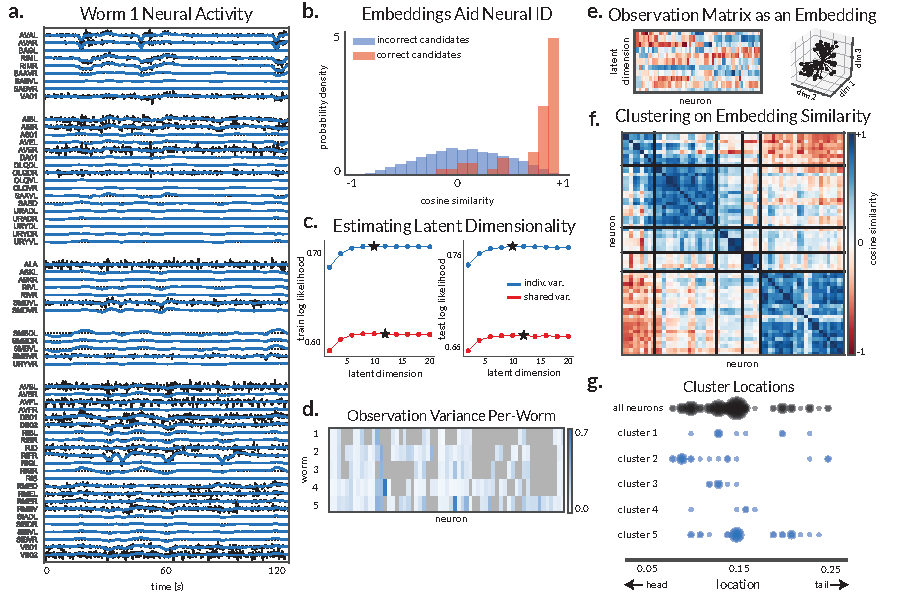
\includegraphics[width=6in]{figures/v4/figure2} 
\caption{ \textit{Hierarchical state space models smooth noisy
    recordings and predict the activity of unseen neurons.}  We show
  the neural activity (differenced Ca++ traces) for two of the
  five worms from the \citet{kato2015global} dataset.  Of these five
  worms, worm 1 (left) has the fewest labeled neurons and worm 5
  (right) has the most.  Green lines are the measured activity of the
  labeled neurons; black lines are the smoothed activities predicted
  by the model for the 61 neurons that were labeled in at least one
  worm.  The model uses correlations learned across all recordings to
  predict the activity of unlabeled neurons, like \textsf{SMBDL} in
  worm 1.  The neurons have been clustered based on similarity, as
  discussed in Fig.~\ref{fig:clustering}.  }
\label{fig:smoothing}
\end{figure}


The parameters of the learned model offer insights into the structure
of neural activity in the head ganglia that can only be obtained by
pooling information across many partial recordings.  We fit our model
to the first-order differences in calcium fluorescence with minimal
preprocessing; we simply correct for photo-bleaching, z-score the
resulting traces, and compute the differences between consecutive
frames. The green lines in Fig.~\ref{fig:smoothing} show a three
minute window of bleaching-corrected, differenced calcium traces for
two of the five worms in the~\citet{kato2015global} dataset. Of these
five worms, worm 1 has the fewest labeled neurons (24 neurons) and
worm 5 has the most (48 neurons). Across the five worms, 61 unique
neuron labels were identified in at least one worm.

By aggregating information across worms, the model learns correlation
structure that enables it to smooth the noisy traces and predict the
activity of unlabeled neurons.  The smoothed and predicted activity
are shown as black lines in Fig.~\ref{fig:smoothing}. For example,
even though \textsf{SMDVR} is not labeled in worm 1, the model
learns how its activity covaries with that of other neurons
by leveraging information from other worms, like worm 5, in which
both~\textsf{SMDVR} and~\textsf{SMDVL} are labeled.  Since these
two neurons are highly correlated, the model makes strong predictions
about the activity of~\textsf{SMDVR} in worm 1 on the basis of the
activity of~\textsf{SMDVL} and other the other observed neurons.

The degree to which the smoothed activity matches the observed
activity is governed by the dimensionality of the latent state space.
We estimate this dimensionality with cross validation, reserving the
last 20\% of the data ($\approx$3.6 min) for testing and measuring the
marginal log likelihood of the held-out data as we increase the latent
dimensionality. We find that the test likelihood is maximized with a
10-dimensional latent state, and that performance improves
substantially after allowing neurons different observation variances
in each worm. This may account for differences in fluorescence level,
for example.

% Moreover, the likelihood is substantially higher in the model that
% includes per-worm observation variances compared to the model with
% shared variances for all worms. Fig.~\ref{fig:supp_emissions}d shows
% the inferred variance for each worm in the \citet{kato2015global}
% dataset.  Neurons that were not identified are marked with a gray box.
% This shows the extent of the missing data and the need for
% hierarchical modeling.\todo{make supplement figure}
 
\subsection*{Emission model reveals clusters of functionally similar neurons}

\begin{figure}[t!]
\centering
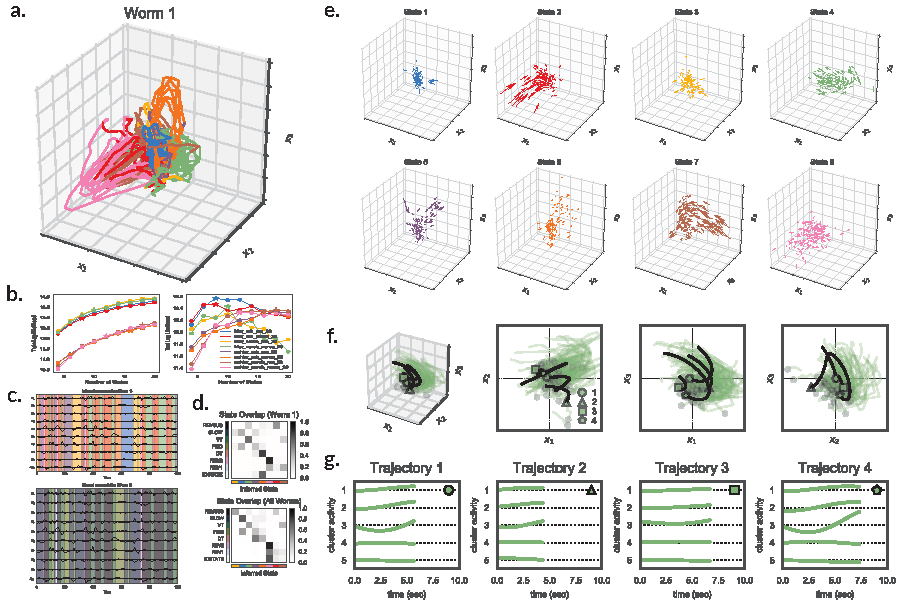
\includegraphics[width=6in]{figures/v4/figure3} 
\caption{ \textit{The mapping from continuous latent states to neural
    activity reveals clusters of functionally similar neurons.}
  \textbf{a.} The emission matrix is a linear map from latent states;
  the rows can be seen as ``tuning vectors'' that specify how each
  neuron responds to changes in the latent state.  These tuning
  vectors cluster into discrete groups (separated by black lines),
  indicating that there are subpopulations of similarly tuned, and
  hence highly correlated, neurons. Neurons are ordered as in
  Fig.~\ref{fig:smoothing}. \textbf{b.}~The pairwise similarity
  between tuning vectors supports this clustering and shows
  differences between subpopulations (clusters have been sorted to
  make this as close to diagonal as possible).  \textbf{c.}~The
  empirical correlation matrix between neurons mimics the similarity
  between tuning vectors, but has a substantial number of missing
  entries (gray, off-diagonal boxes) for pairs that were never
  simultaneously recorded .  \textbf{d.}~We show the spatial locations
  of neurons from each cluster, as specified by WormAtlas.  Neurons in
  the same cluster are not necessarily close to one another in space,
  though some clusters are spatially localized. Black bars denote
  approximate locations of the anterior (AG), dorsal (DG), ventral
  (VG) and retrovesicular ganglia.  \textbf{e.}~Clusters 2 and 7
  contain only sensory (S) neurons, but the other clusters contain
  neurons with a mix of interneurons (I), motor (M) and polymodal (P) neurons, and
  neurons of unknown (U) type. \textbf{f.}~However, these clusters of
  interneurons and motor neurons are functionally grouped, according
  to expert labels. }
\label{fig:clustering}
\end{figure}


The linear mapping from latent states to observations reveals clusters
of similarly tuned neurons.  The mapping is given by a matrix with
rows corresponding to neurons and columns corresponding to latent
dimensions, shown in Fig.~\ref{fig:clustering}a.  Each row can be seen
as a \emph{tuning vector} that specifies how the corresponding neuron
responds to each dimension of the latent state.  This matrix reveals
groups of similarly tuned neurons. To capture these groups, we used
k-means to cluster the neurons based on their tuning vectors and found
that 12 clusters adequately captures the diversity of the population.
Using fewer clusters leads to qualitatively similar groups but omits
some of the finer within-group differences; allowing more clusters
eventually leads to groups of lateral pairs (like \textsf{ASKL} and
\textsf{ASKR} in Fig.~\ref{fig:clustering}a).  The neurons are ordered
as in Fig.~\ref{fig:smoothing}, and clusters are separated by black
lines.

Fig.~\ref{fig:clustering}b shows the cosine similarity of tuning
vectors for each pair of neurons, illustrating the differences
and similarities between clusters.  We notice two prominent
features.  First, the block structure of this
matrix lends support to the notion of discrete clusters, indicating
strong similarity between neurons within the same cluster. Second,
we have sorted the clusters in order to make this matrix as
diagonal as possible.  Upon doing so, we see a banded structure
indicating that in addition to the discrete clustering, there is
also a continuum along which these clusters vary, with the first
clusters more similar to each other than to the latter clusters.
Since the diagonal values equal one by definition, these
have been grayed out. 

In our model, the emission matrix determines the correlations between
neurons.  As such, we expect the similarity between rows of the
emission matrix to mimic the empirical correlations observed in the
data.  Fig.~\ref{fig:clustering}c shows that this is indeed the case,
as neurons with similar tuning vectors also have higher empirical
correlation coefficients.  However, without a hierarchical model, we
cannot empirically estimate the correlation between pairs of neurons
that were not simultaneously observed.  For this dataset, this leaves
many entries in the empirical correlation matrix missing, as denoted
by the gray off-diagonal entries. A key advantage of our hierarchical
model is its ability to draw inferences in the face of significant
amounts of missing data.

What can explain this clustering?  We first look at the spatial
locations of neurons in each cluster, under the hypothesis that
clusters could be trivially explained by an inability to resolve
differences in activity between nearby neurons.
Fig.~\ref{fig:clustering}d shows the locations of all 61 labeled
neurons, using the positions from WormAtlas \citep{wormatlas} along the
head-tail axis of the worm's body.  The size of the dot indicates the
number of neurons at that location; the bars below denote the
approximate location of the anterior (AG), dorsal (DG), ventral (VG)
and retrovesicular (RVG) ganglia.  Some cluster (e.g. cluster 6) are
spatially localized, but many clusters contain neurons from multiple
head ganglia.  This suggests that location alone cannot explain the
similarity between tuning vectors.

Next, we considered the types of cells contained in each cluster.
Fig.~\ref{fig:clustering}e shows the composition of each cluster in
terms of sensory (S), inter (I), motor (M), polymodal (P) and unknown
(U) neuron types.  Clusters 2 and 7 consist of only sensory neurons,
cluster 3 contains mostly interneurons, and clusters 8 and 11 are
primarily motor neurons, but the other clusters are composed of a mix
of inter and motor neurons. Thus, cell type alone appears insufficient to
explain these clusters as well. 


\subsection*{Model predictions aid in neural identification}

\begin{figure}[t!]
\centering
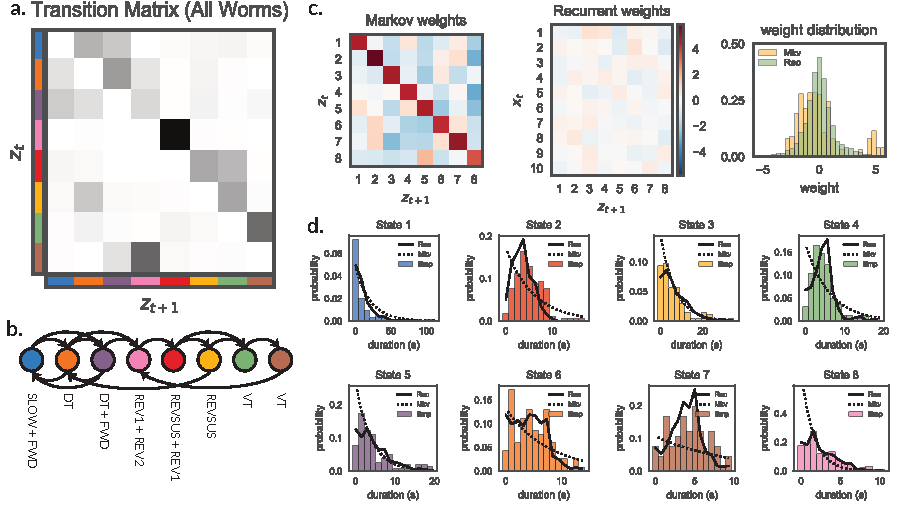
\includegraphics[width=6in]{figures/v4/figure4} 
\caption{ \textit{The predicted neural activity is a useful aid for
    neural identification.}  \textbf{a.} The model uses observed and
  labeled activity (green traces) to predict the activity of unlabeled
  neurons, as in Fig.~\ref{fig:smoothing}. \textbf{b.} Alongside the
  labeled activity, we also have traces from many neurons that could
  not be labeled with certainty. To test whether the model's
  predictions could aid in labeling neurons, we conducted a synthetic
  experiment, withholding the activity of some labeled neurons. Here,
  the red trace is the withheld activity of VB01 and the blue traces
  are the activity of other unlabeled neurons.  Together, these make
  up a pool of candidates for the VB01 label.  \textbf{c.} For each
  candidate, we measured the correlation between its activity and the
  predicted activity of VB01.  \textbf{d.} Repeating this experiment
  50 times, we found that the correct candidates tend to be much more
  correlated with the model's predicted activity than the other,
  incorrect candidates.  Thus, the model's predictions serve as a
  useful aid for labeling neurons.  }
\label{fig:id}
\end{figure}

The predicted activity is based on the correlations between neurons
learned from many recordings.  These predictions should be a useful
aid for laneling neurons whose activity could be measured but whose
identity could not be unambiguously resolved.  To test this
hypothesis, we conducted a synthetic experiment in which we withheld
the labels of ten neurons per worm.  We fit the model to the remaining
neurons and then compared the model's predicted activity to the
activity of the heldout neurons, as well as to the activity of the
unlabeled neurons identified by~\citet{kato2015global}.

Fig.~\ref{fig:id}a shows a schematic of the experiment: though VB01
was labeled in the dataset, we withheld its activity and used the
model to predict it (black trace) based on the observations of the
other, labeled neurons (green traces).  We then compared the model
predictions to the true activity of VB01 (red trace) and to the
activity of other neurons that were recorded but could not be labeled
(blue traces), as shown in Fig.~\ref{fig:id}b.  We computed the
correlation coefficient between these traces and the predicted
activity of VB01, as shown in Fig.~\ref{fig:id}c.  In this case, the
model's predictions and the true activity are highly correlated, even
though the true activity was not used when training the model.  We
repeated this experiment for 50 heldout neurons and found that this
pattern holds: the predicted activity is typically much more
correlated with the activity of the correct heldout trace (red
histogram) than with the activity of other unlabeled neurons (blue
histogram).  This suggests that our hierarchical model may serve an
additional role in aiding neural identification in ambiguous, noisy
data.

Table~\ref{tab:neuron_id} shows the results of a more challenging, yet
more realistic experiment.  Here we withheld the identities of ten
neurons at a time in each worm.  We combined the activity of these
neurons with those of the other measured but unlabeled neurons to form
a candidate pool that ranged from 76 neurons to 111 neurons in size.
Then we solved a minimum weight bipartite matching problem to
simultaneously match the candidates to the set of all possible labels
(which consists of 23 to 47 possible labels, not just the ten that
were artificially withheld).  We find that in all five worms, 6 to 8
of the 10 withheld labels were accurately matched.  While this is
impressive performance for this challenging task, we expect that
further improvements could be obtained with recent work on variational
Bayesian inference for permutation and matching inference
problems~\citep{linderman2018reparameterizing}.


\subsection*{SLDS automatically parse data into discrete, behaviorally meaningful states}

\begin{figure}[t!]
\centering
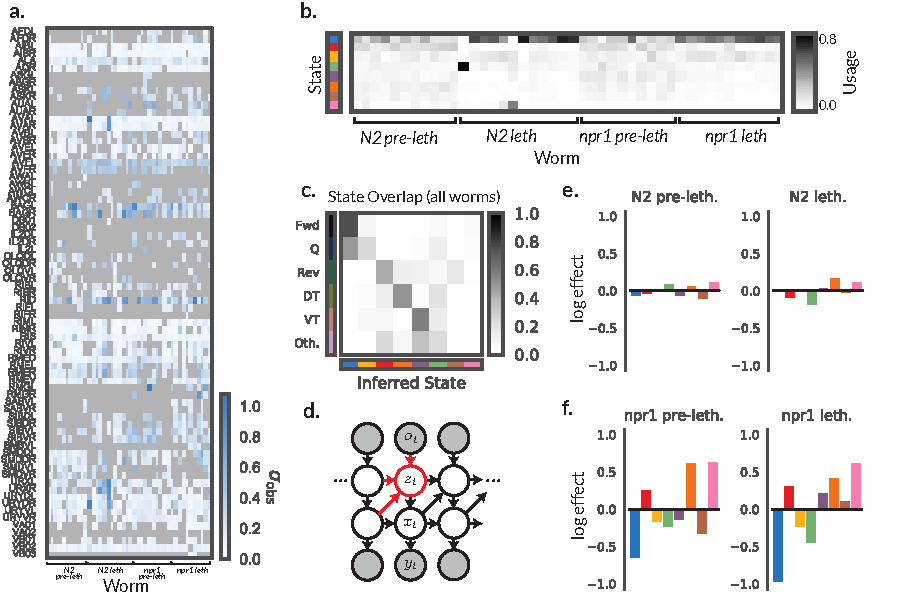
\includegraphics[width=6in]{figures/v4/figure5} 
\caption{ \textit{The hierarchical SLDS automatically segments neural
    activity based on its dynamics.}  \textbf{a.}~The top three
  dimensions, according to variance explained, of the inferred
  continuous latent states for each of the five worms, color coded by
  the corresponding discrete syllable.  \textbf{b.}~The same
  continuous latent states but now color coded according to the manual
  segmentation of~\citet{kato2015global}.  \textbf{c.}~The inferred
  segmentations (top) and the manual segmentations (bottom) over time
  for worm 5. The segmentations largely align, though some manually
  labeled states are split into multiple inferred states (e.g. forest
  green state is often split into green and brown) and others are
  combined (e.g. light purple, light blue, and white are often
  combined into pink).  \textbf{d.}~We quantified the overlap between
  the manual and inferred states and found a close correspondence.
  As~\citet{kato2015global} showed, the manually labeled states map
  onto different behaviors (\textsf{REVSUS}: sustained reversal;
  \textsf{SLOW}: slow forward crawl; \textsf{VT}: ventral turn;
  \textsf{FWD}: forward crawl; \textsf{DT}: dorsal turn; \textsf{REV1,
    REV2}: reversals; \textsf{NOSTATE}: undetermined). The
  correspondence between inferred and manually labeled states shows
  that hierarchical state space models can infer behaviorally
  meaningful states directly from neural activity.}
\label{fig:syllables}
\end{figure}

Having learned a mapping from latent state space to observed activity,
we can now study the dynamics of these continuous latent
states. Fig.~\ref{fig:syllables}a plots the trajectory of the first
worm's neural activity in the top three dimensions of the continuous
state space, color coded by the discrete regime inferred under the
SLDS.  These are the three dimensions with the highest percentage of
expained variance. We see that different regimes correspond to
distinct loops through latent space.  Compare this with Fig. 4b
of~\citet{kato2015global}---they achieved a similar result by manually
segmenting smoothed trajectories in the space spanned by the first
three principal components.  In contrast, our probabilistic framework
is automatic, operates on ten-dimensional latent states, combines
recordings across worms, and requires no additional preprocessing of
the data.

We use the likelihood of held-out test data to determine the number of
discrete syllables and assess the value of the robust and recurrent
model extensions, as shown in Fig.~\ref{fig:model_selection}.  Across
the board, we see a significant improvement when moving from a single
syllable, which is equivalent to an autoregressive model, to multiple
syllables.  Likewise, we see substantial improvements when adding the
robust and hierarchical extensions.  Moreover, in the hierarchical and
robust models, we see a further improvement by introducing the
recurrent extensions.  The test likelihood is maximized with
eight latent states, which matches the number manually chosen
by~\citet{kato2015global}.

Not only does the SLDS find the same number of states, it also finds a
close correspondence between the manually labeled and inferred states.
Fig.~\ref{fig:syllables}b shows ten-dimensional latent states and the
manual and inferred segmentations for a three minute section of data.
The manual and inferred states often change at similar times. We also
see instances where there appears to be a change in continuous state
dynamics that are identified by the SLDS before it is detected in the
manual segmentation (e.g. around 11.8 min).  Fig.~\ref{fig:syllables}c
quantifies the overlap in states for the first worm and for all worms.
Many inferred states are in one-to-one correspondence with manually
labeled states. Some manual states are split into two inferred states
(e.g. ventral turns (\textsf{VT}) are split into green and brown) and
others are combined (e.g. reversals and undetermined states
(\textsf{REV1}, \textsf{REV2}, \textsf{NOSTATE}) map onto pink).
The correspondence between manual and inferred states shows that
the hierarchical SLDS is a useful tool for automatically segmenting
brain data into behaviorally meaningful states.


\subsection*{Syllable dynamics differentially activate clusters of neurons}

\begin{figure}[t!]
  \centering
  \vspace{-.5in}
  \includegraphics[width=6in]{figures/v4/figure6B}
  \caption{\textit{Discrete syllables are characterized by simple
      linear dynamics that give rise to interpretable patterns of
      neural activity.}  \textbf{a.}~Each syllable is associated with
    a canonical set of linear dynamics, which can be viewed as
    mappings from~$\reals^{10}$ to~$\reals^{10}$.  We show the
    mappings for the first three dimensions here, with colored arrows
    placed at locations where each syllable was used.  The black
    arrows show a simulated trajectory with the syllable's
    dynamics. The syllables are ordered by their overall usage, with
    syllable 1 being used most and syllable 8 least. \textbf{b.}~We
    mapped the simulated latent state trajectories (black arrows in
    a.) through the emission matrix to compute a time course of
    resulting activations for each cluster of neurons.  \textbf{c.}
    Using 1000 simulations, we computed the average activation each
    syllable gives rise to on each cluster, as well as the average
    change in activation.  }
  \label{fig:dynamics}
\end{figure}

The hierarchical SLDS not only automates the laborious manual
segmentation process, it justifies the segmentation with a
quantitative definition of each inferred syllable. Each syllable is
associated with a set of canonical linear dynamics, as shown in
Fig.~\ref{fig:dynamics}a. The colored arrows in these vector fields
show how the continuous state in one time bin is mapped to a new
location in the next time bin according to the corresponding discrete
syllable (for the top three latent dimensions).  Arrows are only drawn
at those locations where the syllable was actually employed.

Syllables 1 (blue), 3 (yellow), and 5 (purple) are all characterized
by convergence toward the origin, which corresponds, essentially, to
no change in neural activity. These three syllables differ in terms of how
quickly they converge to the origin and the amount of rotation as
they do so.  By contrast, syllables 2 (red), 4 (green), 6 (orange), 7(brown)
and 8 (pink) form parts of rotational loops in latent state space.
As the latent state traces out a loop, it transiently activates
the clusters of neurons that are tuned to the loop direction.
These states are associated with dorsal turns, ventral turns, and
reversals.  

We use these dynamics to simulate how brain activity evolves under the
different syllables. The black arrows in Fig.~\ref{fig:dynamics}a show
one simulated trajectory for each syllable. Fig.~\ref{fig:dynamics}b
shows how these simulated trajectories map into activations in the
space of neural activity. For each discrete
syllable, we chose the starting locations randomly from the set of
locations where that syllable was entered in the real data.  We then
simulated forward in time according to that syllable's dynamics until
the simulation predicted a transition to another syllable.  We then
mapped these simulations for each state through the emission
matrix and measured the average activation induced on each of the 12
neural clusters.

These activations lend further evidence in support of the behavioral
labels attributed to each state. For eaxample, state 4 (green)
coincides with the manually labeled ``ventral turn'' state.  Its
dynamics produce a pronounced rise and fall in the activity of cluster 6, which
(referring back to Fig.~\ref{fig:clustering}), consists of the
\textsf{RIVL/R} and \textsf{SMDVL/R} neurons.  The \textsf{RIV} pair
are polymodal inter- and motor-neurons that specify the ventral bias
of turns, and the \textsf{SMDV} are motor neurons that initiate
ventral turns.  We also see that states 6 (orange) and 5 (purple) often
produce a dip followed by a rise, respectively, of activation on cluster 8,
which together produce a dorsal turn.
\todo{Need confirmation of these results.  Hard for me to tell difference between
dorsal turn activation (orange to purple) and ventral turn (green to brown).}

To understand the overall effect of these different syllables, we
simulated 1000 continuous latent state trajectories for each, with
the same procedure as above.  We again mapped these into neural space
and computed the activation of each cluster.  We averaged over all
the simulations to compute the average cluster activation shown in
Fig.~\ref{fig:dynamics}c (left).  We did the same with the difference
between starting and ending activation to compute the average change
in cluster activation shown in Fig.~\ref{fig:dynamics}c (right).
We notice that different subsets of clusters tend
to be activated by different syllables.  In other words, syllables
engage unique subsets of neurons. 

\subsection*{Recurrent models learn spatially localized syllables and non-Markovian transitions}

\begin{figure}[t!]
\centering
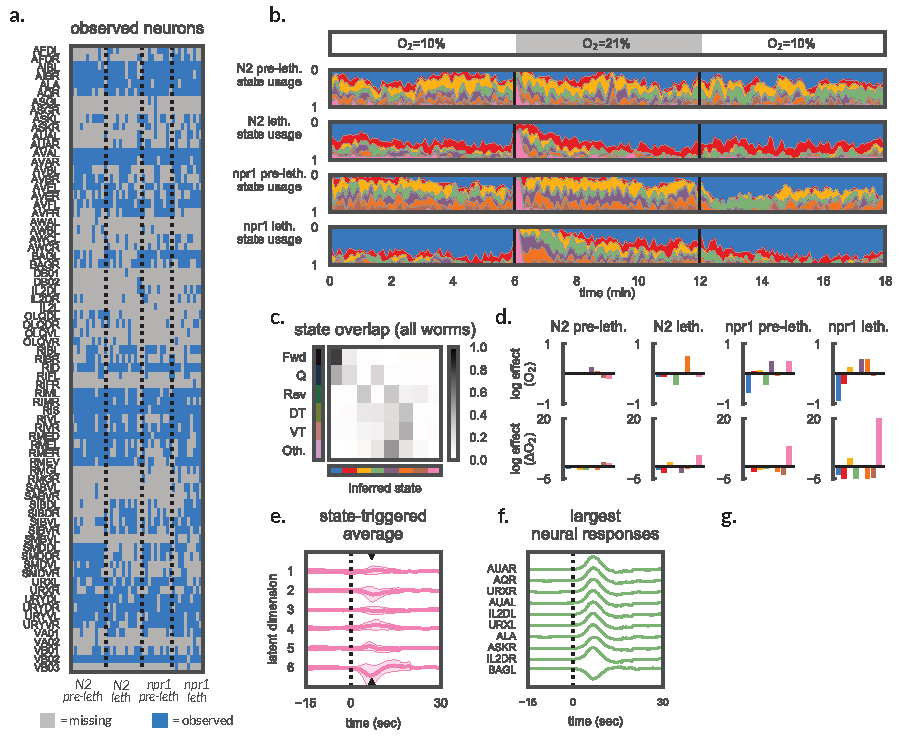
\includegraphics[width=6in]{figures/v4/figure7} 
\caption{ \textit{Discrete syllable transitions show a chain-like
    structure with non-Markovian durations.}  \textbf{a.}~Counts of
  inferred transitions from one syllable to another. The syllables are
  permuted to emphasize the feed-forward structure.  \textbf{b.}~An
  alternative view of the transitions; each syllable is a node in a graph
  and edges denote high-probability transitions.  This shows
  transitions between forward and reverse crawling linked by dorsal
  and ventral turns.  \textbf{c.}~The standard SLDS assumes Markovian
  transitions, which imply a geometric distribution of syllable durations
  (dotted black lines), but Fig.~\ref{fig:syllables} suggests that
  transitions occur near the origin.  With the exception of
  syllable 7, which is unstable, the recurrent SLDS incorporates this
  dependency and generates syllable durations (solid black lines) that
  are a better fit to those inferred from the data (colored bars).  }
\label{fig:recurrent}
\end{figure}

The final component of our hierarchical state space model is the
discrete transition distribution.  In contrast to standard SLDS, we
allow these transition probabilities to depend on the location in
continuous state space (via the \emph{recurrent} dependency) as well as
the preceding discrete syllable (the \emph{Markovian} dependency).
Fig.~\ref{fig:recurrent}a shows the contribution of the Markovian
term.  Each cell in this matrix denotes the number of transitions from
one syllable to another. We are only counting transitions in which the
syllable changes, hence the diagonal is zero.  We have permuted the
syllables to emphasize the largely feed-forward structure.

Fig.~\ref{fig:recurrent}b shows the strongest entries in this matrix
in an alternative form.  We have illustrated each state as a node in a
graph, and labeled the states based on their correspondence with the
manually labeled states of~\citet{kato2015global} (see
Fig.~\ref{fig:syllables}d).  This reveals a chain-like transition
structure in which slow and forward (\textsf{FWD}) crawling are linked
to reverse (\textsf{REV1}, \textsf{REV2}) and sustained reverse
(\textsf{REVSUS}) via dorsal turns (\textsf{DT}). From sustained
reverse crawling, the worm may execute either dorsal or ventral turns
(\textsf{VT}).

Though these syllables were inferred from neural activity alone, the
transition structure---forward and reverse crawling linked by dorsal
and ventral turns---mimics the natural behavior of freely crawling
worms.  This point was made by~\citet{kato2015global} based on their
manual segmentation of neural activity; here we see that this finding
holds given our automatic segmentation as well.  Moreover, we obtain
further insights by studying the precise transition structure that
links these syllables together according to the current syllable
as well as the current continuous latent brain state. 

To accurately model the transitions between syllables, the changes
must occur at specific boundaries in continuous latent space.  Namely,
Fig.~\ref{fig:syllables}a shows that the loops tend to start and end
at the origin, and we rarely see transitions when the continuous
latent state is far from zero. This manifests in signature duration
distributions for the various states.  Fig.~\ref{fig:recurrent}c plots
these distributions for each of the eight states.  Superimposed on
top, we show the predicted distributions with the recurrent SLDS
(solid black lines) compared with the predictions of the standard,
Markovian SLDS (dotted black lines). The Markovian model knows nothing
of the continuous latent state and implies a geometric duration
distribution with monotonically decreasing probability. By contrast,
the recurrent model learns to transition near the origin, which gives
rise to characteristic duration distributions that closely match the
empirical distributions.


\subsection*{Oxygen level modulates transition probabilities but not dynamics or emissions}

\begin{figure}[t!]
\centering
\includegraphics[width=6in]{figures/v4/figure8} 
\caption{\textit{Incorporating exogenous factors like oxygen level
    into the dynamics model reveals how external covariates
    differentially modulate transition probabilities in worms of
    different genetic strains and developmental stages.}
  \textbf{a.}~The observed neurons variances for each of the 41 worms
  in the~\citet{nichols2017global} dataset.  \textbf{b.}~Worms of
  different genetic strains (N2, npr1) and developmental stages
  (pre-lethargus, lethargus) exhibit different average syllable usages
  as a function of the oxygen level.  Blue and red syllables are much
  more likely in the lethargus stage for both genetic strains, but
  they are suppressed in npr1 worms at high (21\%) oxygen
  concentrations. Moreover, we see a pronounced increase in the pink
  syllable usage immediately after the oxygen level increases to 21\%.
  \textbf{c.}~As above, the inferred states closely match the manually
  labeled states of~\citet{nichols2017global}, with blue, red, and to
  a lesser extent green mapping onto the forward (\textsf{Fwd}) and
  quiescent (\textsf{Q}) states.  \textbf{d.}~We extended the model to
  incorporate oxygen level (O$_2$) and change in oxygen level
  ($\Delta$O$_2$) as exogenous factors that drive discrete transition
  probabilities.  We find that oxygen level has a limited effect on N2
  worms but strongly suppresses the blue (\textsf{FWD/Q}) state in
  npr1 worms and promotes the purple and orange
  (\textsf{Rev/DT/VT/Other}) states. The largest effect arises from
  the change in oxygen: an increase in $O_2$ strongly elicits the pink
  syllable.  \textbf{e.} The average continuous latent state
  trajectory following entry into the pink syllable shows a dip in
  activity along the last dimension 7 seconds after entry (black
  arrows).  \textbf{f.} This dip gives rise to strong excitatory
  responses of sensory neurons \textsf{URXL/R} and \textsf{AUAL/R}
  (among others), which are known to respond to increases in oxygen
  concentration. Likewise, we see strong inhibition of other neruons,
  like the chemosensory neurons \textsf{ASGL/R} and \textsf{BAGL/R}.}
\label{fig:o2}
\end{figure}

The preceding results demonstrated the efficacy of hierarchical,
recurrent, and robust SLDS for learning interpretable dynamics of
neural activity from the noisy, partial recordings
of~\citet{kato2015global}.  We now turn to the dataset studied
in~\citet{nichols2017global}. It contains many more worms, but it has
roughly the same number of neurons per recording.  However, the
experimental design is more complicated.  First, there are two strains
of worms (N2 and npr-1) at two different stages of development
(pre-lethargus and lethargus); second, the oxygen concentration is
manipulated over the course of the recordings to elicit different
responses.  Here we show how our framework can be extended to study
the effects of these manipulations.

Fig.~\ref{fig:o2}a shows the neurons that were labeled in each of the
recordings. There are 41 worms, roughly ten from each strain and
developmental stage combination (N2 + pre-lethargus, N2 + lethargus,
npr1 + pre-lethargus, and npr1 + lethargus). Some neurons are
consistently identified in almost all worms; others are identified in
only a handful.  As before, our hierarchical framework combines all
this information to learn a canonical dynamical system.

Upon fitting our model, we immediately see a difference in the average
usage of the eight syllables as a function of oxygen
level(Fig.~\ref{fig:o2}b). The worms in the lethargus stage
predominantly use the blue and red syllables.  Again, we found a close
correspondence between our inferred syllables and the manually labeled
states of~\citet{nichols2017global} (Fig.~\ref{fig:o2}c). Here, blue
and red both map strongly onto the quiescent (\textsf{Q}) state. This
is consistent with the characterization of the lethargus stage---at
this stage, worms exhibit much less crawling behavior. The
pre-lethargus worms execute a broader variety of behaviors, including
reversals (\textsf{Rev.}) and dorsal and ventral turns (\textsf{DT}
and \textsf{VT}, respectively).

A key finding of~\citet{nichols2017global} was that increasing the
oxygen level elicits activity in lethargus npr1 worms but not in
lethargus N2 worms. We quantify this effect with our models by
including oxygen level (O$_2$) and change in oxygen level ($\Delta$O$_2$)
as exogenous inputs.
% Fig.~\ref{fig:o2}d
% shows how the graphical model of the recurrent SLDS changes: now the
% discrete state at time~$t$ (red circle) depends on the preceding discrete
% state, the preceding continuous state, and the current oxygen level.
% \todo[inline]{consider alternative models in which oxygen level
%   influences continuous states and observations?}
Fig.~\ref{fig:o2}d (top) shows the inferred effect of oxygen level for
each of the four strain/developmental stage pairs.  As predicted,
higher oxygen levels increase the probability of reversals and turning
related states (orange, purple) and decrease the probability of
forward and quiescent (blue, red, green) states in npr1 worms, but has
limited effect on N2 worms.  Somewhat surprisingly, the magnitude of
the effect is comparable for both pre-lethargus and lethargus npr1
worms, even though the baseline level of reversals and turns is much
higher in the pre-lethargus worms.

The largest effect is in response to the change in oxygen level, as
shown in Fig.~\ref{fig:o2}d (bottom).  Across all worms, the change
from 10\% to 21\% oxygen concentration sharply increases the probability
of transitioning into the pink syllable. Moreover, this syllable is seldom
used except for when the oxygen level increases.  This suggests that
sharp increases in oxygen level induce a transient and characteristic
neural response in worms of both genetic strains and developmental stages,
however the sustained upregulation of active states in response to elevated
oxygen concentration is unique to npr1 worms.

Fig.~\ref{fig:o2}e shows the average latent state trajectory triggered
upon entry into the pink syllable (for this dataset, the optimal
performance was achieved by a 6-dimensional continuous late state
space).  We see a dip and rebound along the last dimension
approximately 7 seconds after entry (denoted by the black arrows).  We
identified the neurons that showed the largest excitatory and
inhibitory responses at this point in time and plotted the top ten in
Fig.~\ref{fig:o2}f and g, respectively.  Unsurprisingly, these neurons
are largely sensory and interneurons.  In particular, \textsf{URXL/R}
and \textsf{BAGL/R} are known to jointly encode changes in oxygen
level with opposing signs: \textsf{URXL/R} respond to increases in
oxygen, \textsf{BAGL/R} respond to dcreases.  Our model recapitulates
these results and suggests that many other sensory neurons respond
similarly to this stimulus.

\clearpage

\section*{Discussion}

\clearpage

\bibliography{refs}
\bibliographystyle{abbrvnat}

\clearpage

\appendix
\counterwithin{figure}{section}
\counterwithin{table}{section}

\section{Data representation and preprocessing}
\label{sec:data}

The data comes in the form of a collection of matrices~$\{\widetilde{Y}^{(w)}\}_{w=1}^W$
for each of~$W$ worms.  The matrix~${\widetilde{Y}^{(w)} \in \reals^{T_w \times N_w}}$
represents the calcium activity of the~$w$-th worm, which consists of~$T_w$
time frames and~$N_w$ neurons.\footnote{Technically, this calcium activity is
a matrix of first-order temporal differences of a
bleaching-corrected~$\Delta F /F$ signal. Unlike~\citet{kato2015global}, we
do not smooth these derivatives. We work with the raw first-order
temporal differences.}  \celegans~is special in that each neuron has a unique
name.  Assigning names to neurons in calcium imaging data is a challenging
task, but typically, out of the~${\sim 100}$ neurons observed in any worm,
we can label about~$20-30$ with high certainty.  As such, we choose to
represent each matrix~$\widetilde{Y}^{(w)}$ in \emph{canonical form} as a
tuple~$(Y^{(w)}, M^{(w)})$, where~${Y^{(w)} \in \reals^{T_w \times N}}$ is
a matrix where each column corresponds to one of the~$N$ neurons that is
identified in at least one of the~$W$ worms, and~${M^{(w)} \in \{0,1\}^{T_w \times N}}$
is a corresponding \emph{mask} matrix that indicates which neurons were
observed in worm~$w$.  If~$M_{:,n}^{(w)} = 1$, neuron~$n$ was labeled in
worm~$w$ and~$Y_{:,n}^{(w)}$ was its observed activity.  If~$M_{:,n}^{(w)}=0$,
this neuron was not observed in worm~$w$, and the corresponding activity
is missing.\footnote{The mask is defined in such a way that neurons can
  be missing for only subsets of time frames, but in our data neurons are
  either labeled or missing.}
% todo: note that we could also (and have also) model the activity of
% unlabeled neurons.  For the final analyses, I'm not doing this though.

\section{Hierarchical state space model for neural data}
\label{sec:slds}

\begin{figure}[t!]
\centering%
\includegraphics[width=5in]{figures/v4/figure1_supp} 
\caption{\textit{Graphical depiction of a hierarchical, robust,
    recurrent, and input-driven switching linear dynamical system
    (SLDS).}  The blue arrow denotes the \textbf{hierarchical}
  component: each worm~$w$ has its own set of
  parameters~$\theta^{(w)}$, which contain the dynamics libraries,
  emission matrix, etc. These are slight perturbations of the same
  global mean parameters~$\theta$.  In some cases, the worm-specific
  parameters are required to equal their global counterparts (as with
  the emission matrix).  Red arrows highlight the \textbf{robust}
  noise model that links~$x_t$ to~$x_{t+1}$.  Green arrows indicate
  the \textbf{recurrent} extension: the next discrete syllable depends
  on both the preceding syllable as well as the preceding continuous
  latent state.  Purple arrows carry the \textbf{input-dependence}:
  the next discrete syllable can also be governed by an exogenous
  input, like the oxygen level or the change in oxygen level. The
  remaining black arrows denote standard dependencies of the SLDS:
  discrete syllables and continuous latent states co-evolve, with the
  syllables specifying the linear dynamics to use when updating the
  continuous latent states.  The observations are a function of these
  underlying latent states.  The only non-standard addition is an
  autoregressive dependency between~$y_t$ and $y_{t+1}$; here, the
  SLDS models only the differences in observed fluoresence value
  between two consecutive frames.  }
\label{fig:graphical_model}
\end{figure}

We model the neural activity with a switching linear dynamical system
(SLDS) with three new extensions: (i)~a \emph{hierarchical} model to
share parameters across worms while also allowing for worm-to-worm
variability; (ii)~a \emph{robust} model for dynamics noise to help
address model misspecification; and (iii)~a \emph{recurrent} model to
capture how continuous latent states influence discrete state
transition probabilities.  We will introduce the SLDS first and then
present each of these extensions in turn.


\subsection{The standard SLDS}
Switching linear dynamical system models (SLDS) break down complex, nonlinear
time series data into sequences of simpler, reused dynamical modes.
By fitting an SLDS to data, we not only learn a flexible nonlinear generative
model, but also learn to parse data sequences into coherent discrete units.

The generative model is as follows. At each time ${t=1,2,\ldots,T}$,
for each worm~$w$,
there is a discrete latent state ${z_t^{(w)} \in \{1,2, \ldots,K\}}$ that
follows Markovian dynamics,
\begin{equation}
  z_{t+1}^{(w)} \given z_t^{(w)}, \{\pi_k\}_{k=1}^K  \sim \pi_{z_t^{(w)}}
  \label{eq:markov_z}
\end{equation}
where ${\{\pi_k\}_{k=1}^K}$ is the Markov transition matrix and
${\pi_k \in [0,1]^K}$ is its $k$th row. 
In addition, a continuous latent state ${x_t^{(w)} \in \reals^D}$ follows
conditionally linear (or affine) dynamics, where the discrete state $z_t^{(w)}$
determines the linear dynamical system used at time $t$:
\begin{align}
  x_{t+1}^{(w)} &= A_{z_{t+1}^{(w)}} x_{t}^{(w)} + b_{z_{t+1}^{(w)}} +  u_t^{(w)},
  &
  u_t^{(w)} &\iid\sim \cN(0,Q_{z_{t+1}^{(w)}}),
  \label{eq:slds_start}
\end{align}
for matrices ${A_k, Q_k \in \reals^{D \times D}}$ and vectors~${b_k\in
\reals^D}$ for~${k=1,2,\ldots,K}$.
Finally, at each time $t$ a linear Gaussian observation $y_t^{(w)} \in \reals^N$
(some entries of~$y_t^{(w)}$ are masked off; recall Section~\ref{sec:data}) is
generated from the corresponding latent continuous state,
\begin{align}
  y_t^{(w)} &= C x_t^{(w)} + d + v_t^{(w)}, & v_t^{(w)} &\iid\sim \cN(0,S),
    \label{eq:slds_end}
\end{align}
for $C \in \reals^{N \times D}$, $S \in \reals^{N \times N}$,
and~$d \in \reals^N$. We denote the rows of~$C$ by vectors~$c_n$.
For simplicity, we assume~$C$,~$d$, and~$S$ to
be shared among all discrete states in our model.  Moreover, we assume
the observation noise is diagonal,
\begin{align*}
  S &= \diag\left(\left[s_{1}, \ldots, s_{N} \right] \right). 
\end{align*}
The system parameters comprise the discrete Markov transition matrix, the
library of linear dynamical system matrices, and the neuron-specific
emission parameters, which we write as
\begin{equation*}
  \theta = \{(\pi_k, A_k, Q_k, b_k)\}_{k=1}^K \cup \{c_n, d_n, s_n\}_{n=1}^N.
\end{equation*}

To learn an SLDS using Bayesian inference, we place conjugate Dirichlet priors
on each row of the transition matrix and conjugate matrix normal
inverse Wishart (MNIW) priors on the linear dynamical system parameters,
Gaussian priors on the rows of the emission matrix,
and inverse gamma priors on the emission noise.
We write this as,
\begin{align*}
  \pi_k &\given \alpha \iid\sim \distDirichlet(\alpha),
  &
  [A_k, b_k], Q_k &\given \lambda \iid\sim \distMNIW(\lambda),
  \\
  [c_n, d_n] &\given \eta \iid\sim \distNormal(\eta),
  &
  s_{n} &\given \eta \iid\sim \mathrm{IG}(\eta).
\end{align*}
where~$[\cdot, \cdot]$ denotes column concatenation, and $\alpha$, $\lambda$,
and~$\eta$ denote appropriate hyperparameters of the transitions, dynamics, and
emissions, respectively.

\subsection{Extensions of the standard SLDS}
\label{sec:extensions}

To better model the \celegans~data, we introduce three extensions
to the standard SLDS.

\paragraph{Hierarchical model to allow limited variability across worms.}
The first extension captures shared patterns across worms while
still allowing for worm-to-worm variability.  We do this in
two ways. First, we allow the dynamics parameters to vary
slightly from worm to worm with the following model,
\begin{align*}
  \mathrm{vec}([A_k, b_k]) &\sim \distNormal(\lambda), \\
  \mathrm{vec}([A_k^{(w)}, b_k^{(w)}]) &\sim \distNormal(\mathrm{vec}([A_k, b_k]), \sigma^2 I), \\
  Q_k^{(w)} &\sim \mathrm{IW}(\lambda).
\end{align*}
This allows worm-specific dynamics parameters~$(A_k^{(w)}, b_k^{(w)})$ but
requires that they not deviate too far from the global mean~$(A_k, b_k)$.
It also allows for worm-specific dynamics noise. 

Second, we allow each worm to have neuron-specific emission variances,
\begin{align*}
  s_{n}^{(w)} & \iid\sim \mathrm{IG}(\eta).
\end{align*}
We may expect, for example, that calcium indicator expression
varies from worm to worm, which in turn could give rise to
different levels of observed activity.  While this could be
modeled as a scaling of the emission matrix, a simpler approach
is to let the noise term capture these different fluctuations.
We could share the global mean of the worm-specific variances,
but we have little reason to expect the~$s_{n}^{(w)}$ and~$s_{n}^{(w')}$
to be correlated under the prior. 

Figure~\ref{fig:graphical_model} illustrates the complete
probabilistic graphical model.  Each worm has a set of discrete
states~$z_{1:T}$, continuous states~$x_{1:T}$, and observations for a
subset of neurons.  The worms share a set of global dynamics
parameters and emission matrices, but they also have worm-specific
perturbations of the global dynamics, as well as worm-specific
observation variances.

\paragraph{Robust dynamics model.}  While the SLDS can capture nonlinear
dynamics by composing simple linear pieces, it is still an approximation
to the true data-generating process.  To account for some of this
model misspecification, we introduce a \emph{robust} extension of the
SLDS by allowing for heavy-tailed noise in the dynamics.  Specifically,
we replace~\eqref{eq:slds_start} with,
\begin{align}
  x_{t+1}^{(w)} &= A_{z_{t+1}^{(w)}} x_{t}^{(w)} + b_{z_{t+1}^{(w)}} +  u_t^{(w)},
  &
  u_t^{(w)} &\iid\sim \mathrm{t}(0, Q_{z_{t+1}^{(w)}}, \nu_{z_{t+1}^{(w)}}),
\end{align}
where~$\mathrm{t}(\cdot, \cdot, \cdot)$ denotes the multivariate-t
distribution.  This distribution has heavier tails than its Gaussian
counterpart; indeed, it can be derived by a mixture of multivariate
Gaussians with a~$\chi^2$-distributed scaling of the covariance matrix. 

\paragraph{Recurrent model of discrete state transition probabilities.}
Finally, we consider a third extension that allows for more complex
transition probabilities.  We replace~\eqref{eq:markov_z} with,
\begin{align}
  z_{t+1}^{(w)} \given z_t^{(w)}, x_t^{(w)}
  &\sim \mathrm{softmax}(r_{z_t^{(w)}} + R x_t^{(w)}),
    \label{eq:recurrent}
\end{align}
where~${r_k \in \reals^K}$ and~${R \in \reals^{K \times D}}$
parameterize a map from previous discrete and continuous states to a
distribution over next discrete states.  The link function is the
softmax function, which exponentiates and normalizes
the~$K$-dimensional argument~${r_{z_t^{(w)}} + R x_t^{(w)}}$.

\paragraph{Input-driven transition probabilities}
todo
\todo[inline]{Detail the model for how transition probabilities depend
  on oxygen and change in oxygen concentration.  Straightforward extension
  of the recurrent model above.}

\section{Model fitting}

We have proposed a variety of Bayesian algorithms for learning the
model parameters~$\theta$ and performing joint inference of the
latent states~$z$ and~$x$~\citep{linderman2017recurrent, linderman2017structure},
but for simplicity, here we treat inference of~$x$ and~$z$ separately.
That is, first we find low-dimensional continuous states to model the
observations~$y$, then we find a set of discrete states~$z$ that best
explain the dynamics in~$x$. We learn the corresponding parameters
at both stages.


To be more specific, first we fit linear dynamical systems to infer
the continuous latent states~$x$ given the observed values of~$y$.
Since many entries of~$y$ are masked off, this requires inference
with missing data.  Under the assumption of diagonal observation
covariance, this inference is straightforward.  We will compare the
standard LDS with the hierarchical LDS, which has worm- and neuron-specific
variances.

Once we have inferred the continuous latent states, we will fit
an autoregressive hidden Markov model (AR-HMM) to~$x$ in order
to infer~$z$ and learn the dynamics parameters~$(A_k, b_k, Q_k)$.
Here, again, we will consider all possible variants of hierarchical,
robust, and recurrent models.

Both fitting procedures use Markov chain Monte Carlo, specifically
block Gibbs sampling, to sample from the conditional distribution
of latent states given parameters and of parameters given latent
states.  We run these algorithms for 1000 iterations, at which
point we find them to have converged on the basis of held-out
log likelihood. 


\begin{figure}[t!]
\centering%
\includegraphics[width=6in]{figures/v4/figure5_supp1} 
\caption{\textit{Model selection on the basis of marginal log
    likelihood of test data.}  We withheld the last 20\% of the
  continuous latent states from each worm in order to compare
  different models.  For each combination of hierarchical
  vs. standard, robust vs standard, and recurrent vs. standard, we
  swept from~$K=2$ syllables to~$K=20$ (from white to purple)
  syllables in steps of size two. We also included the special case
  of~$K=1$ (grey bars), which reduces to standard autoregressive
  models. For each combination, we fit the model and evaluated the
  marginal likelihood of the held-out test data. The best-performing
  model was the hierarchical, robust, recurrent SLDS with $K=8$
  syllables.}
\label{fig:model_selection}
\end{figure}

We choose the dimensionality of the continuous latent state space
and the number of discrete syllables using the log likelihood of
held-out test data, marginalizing over the corresponding latent
states.  Since we have split inference into two steps, this amounts
to computing the marginal likelihood in a linear dynamical system (LDS)
and an autoregressive hidden Markov model (AR-HMM), respectively.
Both model classes admit efficient marginal likelihood computation
with simple message passing algorithms. Fig.~\ref{fig:model_selection}
shows the held-out log likelihoods used to select the number of
syllables and to justify the hierarchical, robust, and recurrent
extensions.


\begin{figure}[t!]
\centering%
\includegraphics[width=6in]{figures/v4/figure5_supp2} 
\caption{\textit{Discrete states carry substantial information about
    continuous latent states.} How much information is carried by the
  discrete syllables alone? In blue we show the mean and two standard deviations of
  the predictive distribution~$p(x \given z)$.  The esimated values of~$x$
  are shown in black. Below we show the inferred syllables~$z$. We see that
  the discrete syllable carry a surprising amount of information about the continuous
  latent states.}
\label{fig:z_predictions}
\end{figure}

Fig.~\ref{fig:z_predictions} suggests that the switching linear model
for the dynamics of the continuous latent states is indeed a good
model.  In blue we show the predictive distribution~$p(x \given z^*)$
where~$z^*$ is a posterior sample of the discrete syllable sequence.
That this predictive distribution (blue) generally places high
probability on the true values of~$x$ (black lines) indicates that the
switching linear model is a good approximation for the continuous
latent brain states.

\clearpage

\section{Simultaneous identification with an entire population of unlabeled neurons}

\begin{table}[h!]
  \caption{\textit{Artificial neuron identification task results.}  In
    each worm we have~$N_{\mathsf{labeled}}$ labeled neurons
    and~$N_{\mathsf{unlabeled}}$ unlabeled neurons. Of the unlabeled
    neurons, 10 had known labels that were held out for this task.  We
    compare the cosine similarity of the unlabeled neuron embeddings
    to the embeddings of the labeled neurons, sort the similarities,
    and compute the rank of each held-out neuron to its true label
    (most similar~=~1; least similar~=~$N_{\mathsf{unlabeled}}$).  We
    use the Hungarian algorithm to find the most likely matching of
    unlabeled neurons to possible labels, and we report the fraction
    of the 10 held-out neurons that were correctly matched~(``Acc.'').
  }
  \vspace{1em}
  \label{tab:neuron_id}
  \centering
  \begin{tabular}{cccccccccccccc}
    \toprule
    & $N_{\mathsf{labeled}}$ & $N_{\mathsf{unlabeled}}$ & \multicolumn{10}{c}{Matching Rank (10 Held-out Neurons)} & Acc. \\
    \cmidrule(r){2-2}
    \cmidrule(rl){3-3}
    \cmidrule(rl){4-13}
    \cmidrule(l){14-14}
    % \midrule
    Worm 1 & 14 & 95 & 7 & 16 & 1 & 1 & 77 & 3 & 2 & 6 & 4 & 2 & 0.60 \\
    Worm 2 & 31 & 76 & 1 & 5 & 1 & 2 & 2 & 4 & 3 & 2 & 1 & 12 & 0.60 \\
    Worm 3 & 20 & 111 & 7 & 66 & 10 & 9 & 1 & 1 & 1 & 1 & 4 & 1 & 0.70 \\
    Worm 4 & 33 & 93 & 1 & 1 & 3 & 1 & 1 & 48 & 1 & 3 & 4 & 2 & 0.60 \\
    Worm 5 & 38 & 91 & 2 & 1 & 1 & 1 & 1 & 2 & 2 & 3 & 4 & 66 & 0.80 \\
    % Worm 1 & 14 & 95 & 10 & 25 & 1 & 1 & 66 & 2 & 1 & 1 & 2 & 1 & 0.30 \\
    % Worm 2 & 31 & 76 & 3 & 1 & 1 & 1 & 1 & 39 & 1 & 1 & 1 & 4 & 0.50 \\
    % Worm 3 & 20 & 111 & 5 & 53 & 3 & 22 & 1 & 2 & 1 & 1 & 1 & 1 & 0.50 \\
    % Worm 4 &33 & 93 & 2 & 1 & 26 & 2 & 1 & 56 & 1 & 1 & 1 & 1 & 0.30 \\
    % Worm 5 & 38 & 91 & 1 & 1 & 1 & 1 & 1 & 2 & 1 & 26 & 1 & 67 & 0.70 \\
    \bottomrule
  \end{tabular}
\end{table}

\todo[inline]{Discuss this experiment in detail because it is a bit complicated but the results are impressive.}

\clearpage

\section{Eigenspectra of the inferred dynamics}
\begin{figure}[t!]
\centering%
\includegraphics[width=6in]{figures/v4/figure6_supp} 
\caption{The eigenspectra of the dynamics matrices
    provide insight into the nature of the states: imaginary eigenvalues
    give rise to rotational dynamics and the magnitude determines
    whether the stability of the dynamics. The arc denotes
    the unit magnitude line; eigenvalues to the left are contractive
    and to the right are expansive. Looking across rows, we
    see how the spectra vary from worm to worm. 
}
\label{fig:eigen}
\end{figure}

Fig.~\ref{fig:eigen} shows the eigenspectra of the linear
dynamics for each worm and each state.  Imaginary eigenvalues give
rise to rotational dynamics, and the magnitude of the eigenvalues
determines whether the state is stable or not.  If the magnitude is
greater than one (outside the unit disk denoted by the black arc),
the dynamics produce exponential growth in the latent state space; if
the eigenvalues are all less than unit magnitude, the dynamics converge
to a fixed point.  As expected, the rotational states do indeed have
more imaginary eigenvalues, and most states have eigenvalues with
magnitude near one.  Some states, like the brown state, have eigenvalues
larger than one, which produce unstable dynamics, though this is
somewhat balanced by the recurrent extensions discussed in the next
section.  Comparing across rows, we see only minor differences from worm
to worm, substantiating our hierarchical modeling assumptions.

\clearpage

\section{Further analysis of~\citet{nichols2017global} data}

\begin{figure}[t!]
\centering%
\includegraphics[width=6in]{figures/v4/figure8_supp1} 
\caption{\textit{Smoothing and prediction of neural responses
    in \citet{nichols2017global} dataset.} Like Fig.~\ref{fig:smoothing},
  this shows a three minute section of data.  We show one instance
  from each combination of N2 vs. npr1 and pre-lethargic vs. lethargic.
  The three minute window has been centered on the 6 minute mark, at
  which point the oxygen level was increased from 10\% to 21\%.  }
\label{fig:nichols_supp1}
\end{figure}

Fig.~\ref{fig:nichols_supp1} shows 3 minute windows of data from
four worms in the~\citet{nichols2017global} dataset, one worm
from each combination of genetic background (N2 vs npr1) and
developmental stage (pre-lethargus vs lethargus). The window is
centered on the 6 minute mark, at which point the oxygen level
was increased from 10\% to 21\%. At this point in time, we see
a transient response in some clusters of neurons, as discussed
in the main text.  We also note that the noise level varies
substantially from one worm to another, motivating the use of
our hierarchical modeling framework.

\begin{figure}[t!]
\centering%
\includegraphics[width=6in]{figures/v4/figure8_supp2} 
\caption{\textit{Inferred continuous latent states for the four worms
    shown in Fig.~\ref{fig:nichols_supp1}.} As in
  Fig.~\ref{fig:syllables}, we show the continuous trajectories
  color-coded by both the inferred syllable sequence and by the manual
  segmentation. We show this for dimensions (1, 2, 3) and (4, 5, 6),
  sorted by percentage of variance explained. Below, we show the total
  overlap between manual and inferred states, averaging over all worms
  of the given genetic strain and developmental stage.  In all cases,
  there is a reasonable mapping between manual and inferred states,
  though it is not as clear-cut as in the~\citet{kato2015global}
  dataset. In particular, the distinction between forward (Fwd) and
  quiescent (Q) is less clear, with both being mapped to the blue
  state.}
\label{fig:nichols_supp2}
\end{figure}

Fig.~\ref{fig:nichols_supp2} shows the 6-dimensional latent state
trajectories for the four worms whose activity was shown in
Fig.~\ref{fig:nichols_supp1}.  As in Fig.~\ref{fig:syllables} in the
main text, we have color coded the trajectories by the inferred
discrete syllables in panels a. and c., and by the manual segmentation
of~\citet{nichols2017global} in panels b. and d.  Panel e. shows the
average state overlap from all worms of the corresponding genetic
background and developmental stage.  Thought the overlap is not as
one-to-one as we saw in the \citet{kato2015global} dataset, we still
see a strong overlap between manually-labeled quiescent (Q) and
forward (FWD) states and inferred blue and red syllables.  Likewise,
reversals (Rev), dorsal turns (DT), and ventral turns (VT) are often
mapped onto the latter syllables.  We note that the pre-lethargus
worms tend to execute many more turns, making these states much easier
to identify in these worms.  As in the main text, the syllbles
are ordered (blue, red, ...)  according to overall usage.  

\end{document}
